%%%%%%%%%%%%%%%%%%%%%%%%%%%%%%%%%%%%%%%%%%%%%%%%%%%%%%%%%%%%%%%%%%%%
%% I, the copyright holder of this work, release this work into the
%% public domain. This applies worldwide. In some countries this may
%% not be legally possible; if so: I grant anyone the right to use
%% this work for any purpose, without any conditions, unless such
%% conditions are required by law.
%%%%%%%%%%%%%%%%%%%%%%%%%%%%%%%%%%%%%%%%%%%%%%%%%%%%%%%%%%%%%%%%%%%%

\documentclass[
  printed, %% This option enables the default options for the
           %% digital version of a document. Replace with `printed`
           %% to enable the default options for the printed version
           %% of a document.
  twoside, %% This option enables double-sided typesetting. Use at
           %% least 120 g/m² paper to prevent show-through. Replace
           %% with `oneside` to use one-sided typesetting; use only
           %% if you don’t have access to a double-sided printer,
           %% or if one-sided typesetting is a formal requirement
           %% at your faculty.
  table,   %% This option causes the coloring of tables. Replace
           %% with `notable` to restore plain LaTeX tables.
  nolof,     %% This option prints the List of Figures. Replace with
           %% `nolof` to hide the List of Figures.
  nolot,     %% This option prints the List of Tables. Replace with
           %% `nolot` to hide the List of Tables.
  %% More options are listed in the user guide at
  %% <http://mirrors.ctan.org/macros/latex/contrib/fithesis/guide/mu/fi.pdf>.
]{fithesis3}
%% The following section sets up the locales used in the thesis.
\usepackage[resetfonts]{cmap} %% We need to load the T2A font encoding
\usepackage[T1,T2A]{fontenc}  %% to use the Cyrillic fonts with Russian texts.
\usepackage[
  main=czech, %% By using `czech` or `slovak` as the main locale
                %% instead of `english`, you can typeset the thesis
                %% in either Czech or Slovak, respectively.
  english, german, russian, czech, slovak %% The additional keys allow
]{babel}        %% foreign texts to be typeset as follows:
%%
%%   \begin{otherlanguage}{german}  ... \end{otherlanguage}
%%   \begin{otherlanguage}{russian} ... \end{otherlanguage}
%%   \begin{otherlanguage}{czech}   ... \end{otherlanguage}
%%   \begin{otherlanguage}{slovak}  ... \end{otherlanguage}
%%
%% For non-Latin scripts, it may be necessary to load additional
%% fonts:
\usepackage{paratype}
\def\textrussian#1{{\usefont{T2A}{PTSerif-TLF}{m}{rm}#1}}
%%
%% The following section sets up the metadata of the thesis.
\thesissetup{
    date          = \the\year/\the\month/\the\day,
    university    = mu,
    faculty       = fi,
    type          = mgr,
    author        = Lukáš Kotol,
    gender        = m,
    advisor       = {RNDr. Miloš Liška, Ph.D.},
    title         = {Autentizační a autorizační infrastruktura pro videokonferenční prostředí},
    TeXtitle      = {Autentizační a autorizační infrastruktura pro videokonferenční prostředí},
    keywords      = {keyword1, keyword2, ...},
    TeXkeywords   = {keyword1, keyword2, \ldots},
    abstract      = {This is the abstract of my thesis, which can

                     span multiple paragraphs.},
    thanks        = {These are the acknowledgements for my thesis, which can

                     span multiple paragraphs.},
    bib           = example.bib,
}
\usepackage{makeidx}      %% The `makeidx` package contains
\makeindex                %% helper commands for index typesetting.
%% These additional packages are used within the document:
\usepackage{paralist} %% Compact list environments
\usepackage{amsmath}  %% Mathematics
\usepackage{amsthm}
\usepackage{amsfonts}
\usepackage{url}      %% Hyperlinks
\usepackage{markdown} %% Lightweight markup
\usepackage{listings} %% Source code highlighting
\usepackage{hyperref}
\lstset{
  basicstyle      = \ttfamily,%
  identifierstyle = \color{black},%
  keywordstyle    = \color{blue},%
  keywordstyle    = {[2]\color{cyan}},%
  keywordstyle    = {[3]\color{olive}},%
  stringstyle     = \color{teal},%
  commentstyle    = \itshape\color{magenta}}
\usepackage{floatrow} %% Putting captions above tables
\floatsetup[table]{capposition=top}
\begin{document}

\chapter{Úvod}
Komunikace prostřednictvím videopřenosů a multimédií hraje v současném světě informačních technologií důležitou roli. Bez těchto moderních komunikačních prostředků si v dnešní době jen těžko dovedeme představit spolupráci v kolektivu, který tvoří osoby nacházející se na různých místech naší planety. Klíčovou vlastností zmíněných videokonferenčních systémů je dostupnost napříč uživatelskými organizacemi, jejichž spolupráci mají usnadňovat. Aby bylo možné propojení rozdílných organizací, je důležité mít videokonferenční platformu s vybudovanou autentizační a autorizační infrastrukturou, která tyto organizace dokáže integrovat. Pokud je autentizační infrastruktura navíc sdílena mezi další poskytovatele služeb, benefity představované platformy organizací a provozovatelů služeb, tzv. federace identit jsou nemalé. Jedná se například o fakt, že poskytovatelé služeb jsou osvobozeni od správy uživatelských údajů a hesel. Správce služby také definuje, jaký typ uživatele smí k jeho službě přistupovat, bez toho aby tyto politiky musel implementovat. Další výhodou federace identit je skutečnost, že uživateli stačí jen jedno přihlašovací jméno a heslo k přístupu ke všem poskytovaným službám. Uživatel přihlašovací údaje navíc vždy zadává na důvěrně známé webové stránce své organizace. V neposlední řadě, v případě kompromitace  přihlašovacích údajů si uživatel může v jednom kroku vygenerovat nové pro celou federaci identit. 

Cílem této diplomové práce je navrhnout a implementovat novou autentizační a autorizační infrastrukturu pro současné video a webkonferenční prostředí, které spravuje sdružení CESNET\footnote{CESNET, \url{www.cesnet.cz}}. Vytvořená autentizační a autorizační infrastruktura je založena na technologii OpenID Connect\footnote{OpenID Connect, \url{www.openid.net/connect/}}  a je integrována do stávající Proxy IdP v infrastruktuře CESNETu. Na novou autentizační a autorizační infrastrukturu jsou navázány služby meetings.cesnet.cz \cite{shongoapi} a Adobe Connect\footnote{Adobe Connect, \url{www.adobe.com/products/adobeconnect.html}}, které také provozuje sdružení CESNET. Zmíněné videokonferenční služby mohou využívat uživatelé z organizací, které patří do České akademické federace identit eduID.cz \footnote{eduID.cz, \url{www.eduid.cz}} a její mezinárodní obdoby eduGAIN \footnote{eduGAIN, \url{www.edugain.org}}. Portál meetings.cesnet.cz slouží uživatelům k rezervaci výpočeních zdrojů a virtuálních místností,v kterých se uskutečňují následné videokonferenční spojení. Komerční platforma Adobe connect, provozovaná na URL connect.cesnet.cz\footnote{Adobe Connect CESNET Webkonference, \url{www.connect.cesnet.cz}}, umožňuje autentizovaným uživatelům uskutečňovat videokonferenční a webkonferenční schůzky v předem rezervovaných virtuálních místnostech. Zmíněná platforma Adobe Connect navíc podporuje textovou diskuzi, sdílení obsahu dokumentů, kreslící tabule a pracovní plochy počítače v prostředí prohlížeče. 

Výsledkem mé práce je plně funkční autentizační a autorizační infrastruktura zprovozněná v produkčním prostředí webkonferenční platformy sdružení CESNET. Vytvořenou autentizační a autorizační infrastrukturu jsem navrhnul a implementoval na serveru shongo-auth.cesnet.cz pomocí technologie OpenID Connect. Implementovaná infrastruktura je integrována do Proxy IdP provozované sdružením CESNET tak, aby autentizovala a autorizovala uživatele, využívající služeb portálů meetings.cesnet.cz a connect.cesnet.cz. Nová implementace oproti původní rozšiřuje způsoby přihlášení o možnosti použít účty společností Google, Facebook a dalších mezinárodních akademických organizací integrovaných do federace identit eduGAIN. Další předností nové implementace je vynechání autorizačního procesu pomocí externí webové služby Perun\footnote{Perun, \url{www.perun-aai.org}}, která poskytovala základní údaje o autentizovaném uživateli. Nyní jsou údaje přihlášeného uživatele zprostředkovány v rámci autentizačního procesu díky technologii OpenID Connect. Novou implementací došlo tedy k významnému zjednodušení složitosti autentizační a autorizační infrastruktury. \par
Text této diplomové práce je členěn následujícím způsobem. První část se věnuje úvodu. Po úvodu následuje druhá kapitola, ve které popisuji návrh infrastruktury autorizačního a autentizačního systému. V třetí kapitole se věnuji použitým technologiím, které jsem využil v rámci implementace diplomové práce. V následující čtvrté kapitole se zabývám popisem implementace. Poslední pátá kapitola shrnuje výsledky mé práce v závěru.  

\chapter{Návrh autorizační a autentizační infrastruktury}
\section{Popis stávající autentizační a autorizační infrastruktury}
Stávající autentizace a autorizace webkonferenční infrastruktury Shongo a Adobe Connect je založena na systémech Shibboleth \footnote{Shibboleth, \url{www.shibboleth.net}} a Perun \footnote{Perun, \url{www.perun-aai.org/}}. Shibboleth je open-source software, který slouží jako autentizační vrstva s jednotným přihlašováním mezi několika systémy. Perun je centralizovaná služba určená pro správu uživatelských údajů. V dosavadní webkonferenční infrastruktuře, byla služba Perun využívána k získání dodatečných informací o autentizovaném uživateli. \par
Infrastruktura využívající systémy Shibboleth a Perun je implementována na serveru shongo-auth.cesnet.cz. Uvedený server tedy odbavuje požadavky uživatelů na přihlášení do webkonferenčních systémů Shongo a Adobe Connect. Po úspěšné autentizaci je uživatel přesměrovám na požadované portály. 

\subsection{Infrastruktura Adobe Connect}
Webkonferenční platforma Adobe Connect využívá k autentizaci a autorizaci systém Shibboleth a interní databázi, ve které si eviduje uživatele. V uvedené databázi si uchovává informace o uživatelích, které získá po úspěšné autentizaci uživatele. Pokud záznam o uživateli v databázi neexistuje, je vytvořen. Jelikož Adobe Connect využívá jen identifikaci, jméno, příjmení a mail autentizovaného uživatele, není potřeba využívat službu Perun.  

\subsection{Infrastruktura Shongo}
Rezervační systém Shongo využívá při přihlašování uživatelů jak Shibboleth, tak webovou službu Perun. Po úspěšné autentizaci následuje získání dodatečných infomací o uživateli. Prvním krokem je zjištění jedinečného identifikátoru v systému Perun, tzv. \textbf{perun\_id}. Tento identifikátor je vyhledán pomocí jména přihlášeného uživatele webovou službou Perun. Jakmile je znán identifikátor \textbf{perun\_id}, vytvoří se další požadavek na webovou službu Perun na získání dodatečných uživatelských údajů. Konkrétně jde o informace o telefonním číslu, jazyku, časové zóně, příslušnosti do organizace a identifikátoru v rámci organizace uživatele.  

\section{Analýza požadavků}
Z konzultací s vedoucím diplomové práce vyplynuly následující požadavky. Jak už bylo uvedeno v úvodu, hlavní podstatou této diplomové práce je vytvoření nové autentizační a autorizační infrastruktury pro služby Adobe Connect a Shongo provozované sdružením CESNET. Požadavkem bylo, aby tato nová autentizační a autorizační infrastruktura byla implementována v souladu se specifikací OpenID Connect  \footnote{OpenID Connect specifikace, \url{www.openid.net/specs/openid-connect-core-1_0.html}}. Nezbytnou součástí implemtace bylo, aby autentizační a autorizační infrastruktura byla navázána na Proxy IdP OpenID Connect, které provozuje sdružení CESNET\footnote{Proxy IdP OpenID Connect, \url{www.login.cesnet.cz/oidc/}}. Proxy IdP je komponenta mezi poskytovatelem služeb a identit, která umožňuje službě aby byla dostupná prostřednictvím různých poskytovatelů identit.  \par
Dalším požadavkem bylo, aby implementace byla zakomponována do stávajícího autentizančního a autorizačního serveru shongo-auth.cesnet.cz. V neposlední řadě byl odstraněn nepotřebný kódu po nevyužitých voláních webové služby Perun.   


\section{Návrh nové infrastruktury}
\chapter{Použité technologie}
V této kapitole popisuji technologie, které jsem použil při implementaci mé diplomové práce. Popis doplňují informace o tom, v které konkrétní části implementace jsem danou technologii použil.
\section{OAuth}
OAuth 2.0 \footnote{OAuth 2.0 RFC, \url{www.tools.ietf.org/html/rfc6749}} je autorizační framework, který umožňuje aplikacím třetí strany získat omezený přístup k HTTP službám. Zmíněný framework představuje autorizační vrstvu, která odděluje role klienta od držitele zdrojů. OAuth 2.0 popisuje následující role: 
\begin{itemize}
    \item \textbf{resource owner} - entita, schopná dát souhlas s přístupem k požadovanému zdroji, většinou koncový uživatel,
    \item \textbf{resource server} - server, uchovávající chráněné zdroje, schopný odpovídat požadavkům přistupujícím k chráněným zdrojům,
    \item \textbf{client} - aplikace, vytvářející požadavky na získání chráněných zdrojů se svolením resource owner,
    \item \textbf{authorization server} - server, vydávající \textbf{access token} pro roli \textbf{client} po úspěšném ověření \textbf{resource owner} a získání oprávnění.
\end{itemize}
\textbf{Access token} je pověření používané k získání přístupu k chráněným zdrojům. 
Schéma komunikace v protokolu OAuthn 2.0 popisuje následující obrázek \hyperref[fig:oauthn]{3.1}. 

\begin{figure}[H]
\caption{Diagram detailu sezení}
\centering
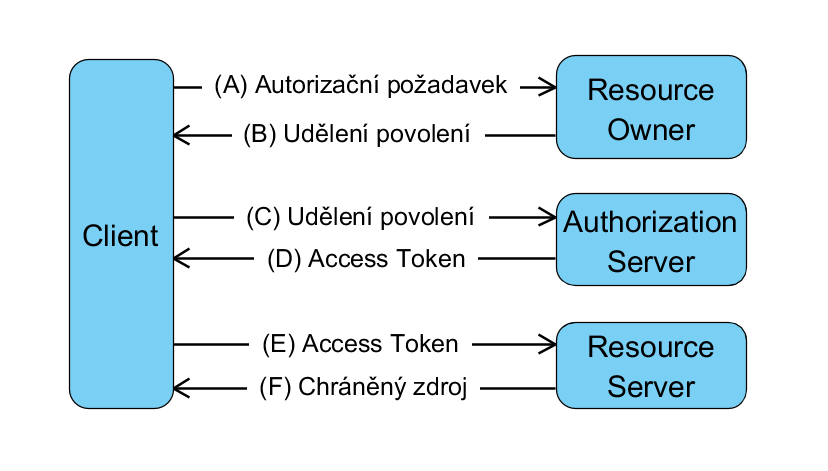
\includegraphics[width=12.8cm]{pics/diplomkaOauth} 
\label{fig:oauthn}
\end{figure}
\par 

V prvním kroku (A) \textbf{client} požaduje autorizaci po \textbf{resource owner}. V další fázi (B) \textbf{client} získá pověření, představující oprávnění vlastníka zdroje. V následujícím kroku (C) \textbf{client} požaduje \textbf{access token} po \textbf{authorization server}, kterému prezentuje udělená oprávnění. Další krok (D) představuje autentizaci a validaci uděleného oprávnění, na základě kterého je vydán \textbf{access token}. V předposlední fázi (E) \textbf{client} přistupuje k \textbf{resource server} s \textbf{access tokenem} a požadavkem na získání chráněného zdroje. Po validaci \textbf{access tokenu} poskytne \textbf{resource server} požadované zdroje entitě \textbf{client} (F). \par 
Jelikož autorizační protokol OAuth 2.0 není navržen pro autentizaci uživatelů a neposkytuje možnost získání dalších informací o přihlášeném uživateli, byl v implementaci použit spolu s technologií OpenID Connect. 

\section{OpenID Connect}
Claim, Scope, Service provider, identity provider, diagram, redirect URL.
autentizace
vrstva nad Oauth
pouziva id token = zakodovany jwt
endpoint pro ziskani informaci o prihlasenem uzivately
standardizovany seznam scope a implementace
slouží k přihlášení 
umožnuje použít 1 učet v ostatních systémech, nejen v tom systému kde byl založen
\section{JSON Web Token}
\section{Apache HTTP server}
Apache HTTP server \cite{apache} (zkráceně Apache) je open-source multiplatformní software, sloužící jako webový server. Apache podporuje velké množství modulů, které rozšiřují základní funkce jádra webového serveru. Hojně využívané moduly podporují použití programovacích jazyků na straně serveru, autentizaci, TLS (Transport Layer Security), SSL (Secure Sockets Layer), proxy a logovací soubory. Konfigurace Apache serveru je založena na souborech \textbf{.htaccess}, v kterých jsou pomocí tzv. direktiv nastavovány pravidla pro zpracování HTTP požadavků. Konfigurace v souboru \textbf{.htaccess} se vztahují pouze na soubory, které jsou umístěné v stejném adresáři jako soubor \textbf{.htaccess} a nebo v jeho podadresářích. Globální konfigurace Apache serveru se standardně realizuje v hlavním konfiguračním souboru \textbf{httpd.conf}. \par
Webový server Apache verze 2 jsem v autentizační a autorizační infrastruktuře využil jako základní prostředek pro zpracování uživatelských HTTP požadavků na přihlášení do videokonferenčních systémů Shongo a Adobe Connect. Konkrétní způsob konfigurace Apache spolu s OpenID Connect modulem popisuji v sekci \hyperref[apacheConfig]{Konfigurace Apache}.

\section{PHP}
PHP \cite{php5} (PHP: Hypertext Preprocessor) je široce používaný open-source skriptovací programovací jazyk, určený především pro tvorbu webových stránek. Zmíněný programovací je multiplatformní, kompatibilní s většinou běžně používaných serverů a podporuje připojení k různým databázovým systémům. Výhodou PHP je rozsáhlý soubor funkcí zabudovaných v základní knihovně, velké množství již vytvořených projektů a kódů, které lze zdarma využít, podpora objektového programování a rozsáhlá dokumentace\footnote{PHP dokuemntace, \url{www.php.net/manual/en/}}. Soubory obsahující zdrojový kód PHP programu jsou standardně označeny příponou \textbf{.php}. \par
V představovaném programovacím jazyce jsem na straně serveru shongo-auth.cesnet.cz implementoval zpracování claims získaných z OpenID Connect po autentizaci uživatele u vybraného Identity providera. Zmíněná implementace je detailněji popsána v kapitolách Implementace autentizačního a autorizačního modulu pro \hyperref[ACImpl]{Adobe Connect} a \hyperref[ShongoImpl]{Shongo}. 

\section{PostgreSQL}
\chapter{Popis implementace}
Popis dostupných claims v Proxy IDP cesnet. 
\section{Instalace OpenID Connect}
\subsection{Konfigurace Apache}
\label{apacheConfig}
\section{Implementace autentizačního a autorizačního modulu pro systém Adobe Connect}
\label{ACImpl}
\section{Implementace autentizačního a autorizačního modulu pro systém Shongo}
\label{ShongoImpl}
\chapter{Závěr}
\printbibliography[title={Literatura}]
\end{document}
